\documentclass[a4paper,12pt]{article}
\usepackage[utf8]{inputenc}
\usepackage{calc}
\usepackage{eso-pic}
\usepackage{graphicx}
\usepackage{parskip}
\usepackage{hyperref}
\usepackage[a4paper,left=25 mm,right=25 mm, bottom=25 mm,
    margin=1in,top=22 mm]{geometry} % Adjusting the margins
\usepackage{tikz}
\usepackage{array}
\usepackage{tabularx}
\usepackage{amsmath}
\usepackage{amssymb}
\usetikzlibrary{calc}

\begin{document}

\begin{titlepage}
\begin{tikzpicture}
    [remember picture, overlay]
    \draw[line width = 2pt, black] 
        ($(current page.north west) + (1cm,-1cm)$) 
        rectangle 
        ($(current page.south east) + (-1cm,1cm)$);
\end{tikzpicture}
    \centering
    \vspace*{0 cm}
    \Large
    \textbf{Maulana Abul Kalam Azad University of Technology, WB}
    \vspace{0.5cm}
    
    
\includegraphics[width=0.3\textwidth]{306-3063564_maulana-abul-kalam-azad-university-logo.png} % Assuming you have the logo image
    \vspace{0.5cm}
    
    \LARGE
    \textbf{\textcolor{blue!60}{Software Tools and Technology\\
        -: Lab Notebook :-}}
    \vspace{0.5cm}
    
    \large
    \textbf{\textcolor{red}{Group 13}}
    \vspace{1 cm}
    
    \textbf{Repository Link:} \href{https://github.com/mishbah-ul-haque/GROUP--13}{https://github.com/mishbah-ul-haque/GROUP--13}
    \vspace{1cm}
    
    \textbf{\underline{\textcolor{blue!60}{Group Members}}}
    \vspace{0.5cm}

    \normalsize
    \begin{enumerate}
        \item \textbf{Sk Mishbah Ul Haque(Leader)}\\
              \textbf{Roll No: 30001223058}\\
              \textbf{Department: BCA}
        \item \textbf{Md Nasim Akhtar}\\
              \textbf{Roll No: 30001223064}\\
              \textbf{Department: BCA}
        \item \textbf{Sreyash Anand}\\
              \textbf{Roll No: 30001223006}\\
              \textbf{Department: BCA}
        \item \textbf{Ritesh Kumar Shah}\\
              \textbf{Roll No: Ritesh Kumar Shah}\\
              \textbf{Department: BCA}
        \item \textbf{Sayantani Hansda}\\
              \textbf{Roll No: 30054623020}\\
              \textbf{Department: BSc in IT (AI)}
    \end{enumerate}
    \vspace{0.8 cm}
    
    \textbf{Instructor:} \href{mailto:ayan.ghosh@university.edu}{\textcolor{blue}{Ayan Ghosh}}\\
    \vspace{0.2cm}
    
    \textbf{\textit{Date: September 11, 2024}}

\end{titlepage}
\newpage
\begin{tikzpicture}
    [remember picture, overlay]
    \draw[line width = 2pt, black]
        ($(current page.north west) + (1cm,-1cm)$)
        rectangle 
        ($(current page.south east) + (-1cm,1cm)$);
\end{tikzpicture}
\vspace{-2cm}

\centering
\section*{\underline{\Huge\textbf{\textcolor{blue!60}{Index}}}}
\vspace{0.5cm}

\renewcommand{\arraystretch}{2}
\setlength{\tabcolsep}{0pt} 

\begin{tabular}{|>{\centering\arraybackslash}p{80pt}|>{\centering\arraybackslash}p{350pt}|}
\hline
\textbf{Serial No.} & \textbf{Questions} \\
\hline
1 & Introduction to GitHub and GitHub Desktop version installation \\\hline
2 & Building a C program for a calculator in the local repository,committing,and publishing it as a public repository \\\hline
3 & Converting a submit button to Chin Tapak Dum Dum \\\hline
4 & Building CV in LaTeX \\\hline
5 & Branching and Merging \\\hline

\end{tabular}

\newpage
\begin{tikzpicture}
    [remember picture, overlay]
    \draw[line width = 2pt, black] 
        ($(current page.north west) + (1cm,-1cm)$) 
        rectangle 
        ($(current page.south east) + (-1cm,1cm)$);
\end{tikzpicture}
\vspace{-2cm}
% Lab notebook entries
\section*{\Huge{\textcolor{blue!60}{Lab Notebook Entries}}}

\subsection*{Entry by Sk Mishbah Ul Haque}
\textit{Date: [\today]}\\
\vspace{1 cm}
\begin{figure}[h!]
   \centering
    
\includegraphics[width=0.5\linewidth]{25231.png}
\end{figure}
\vspace{0.5 cm}

\section*{\Huge{\underline{{-:GitHub:-}}}}
\paragraph{\noindent}{GitHub is a web-based platform that allows developers to host, share, and collaborate on software projects. It provides a version control system powered by Git, enabling teams to track changes, manage code repositories, and work together seamlessly across different locations. GitHub supports collaborative development through features like pull requests, issues, and project boards, making it essential for open-source projects and professional software development. Additionally, it integrates with various development tools, enhancing productivity and streamlining the software development lifecycle.}

\subsection*{\underline{-:Installation:-}}
\paragraph{\setlength{\parindent}{0pt}}{Installing GitHub Desktop is a straightforward process that enhances your workflow by providing a user-friendly interface for managing repositories. To begin, download the installer from the [official GitHub Desktop website](https://desktop.github.com/) for your operating system—Windows or macOS. After downloading, run the installer and follow the on-screen instructions to complete the setup. Once installed, launch the application and sign in with your GitHub credentials, or create a new account if needed. GitHub Desktop simplifies the process of cloning repositories, making commits, and managing branches, making it an invaluable tool for developers of all skill levels. For Linux users, alternative methods like using Wine or other Git clients are available.}

\subsection*{Entry by Md Nasim Akhtar}
\textit{Date: [\today]}\\


\section*{Creating a GitHub Repository and C Calculator Program}

\subsection*{Step 1: Download and Install GitHub Desktop}
1. Go to the GitHub Desktop Website: Visit \texttt{https://desktop.github.com/} and download the installer for your OS.\\
2. Install the Application: Run the installer and follow the instructions.\\
3. Log In: Open GitHub Desktop and log in with your GitHub account.

\subsection*{Step 2: Go Through the Tutorial}
1. After logging in, GitHub Desktop may prompt you for a tutorial.\\
2. Pay attention to how to publish a repository.

\subsection*{Step 3: Create a Local Repository}
1. Click on \texttt{File} and choose \texttt{New Repository}.\\
2. Fill in repository details: 
   \begin{itemize}
       \item Name: e.g., \texttt{C-Calculator}.
       \item Local Path: Choose a location.
   \end{itemize}
3. Click \texttt{Create Repository}.

\subsection*{Step 4: Write a Simple C Program for a Calculator}

\vspace{1 cm}
\begin{figure}[h!]
   \centering
    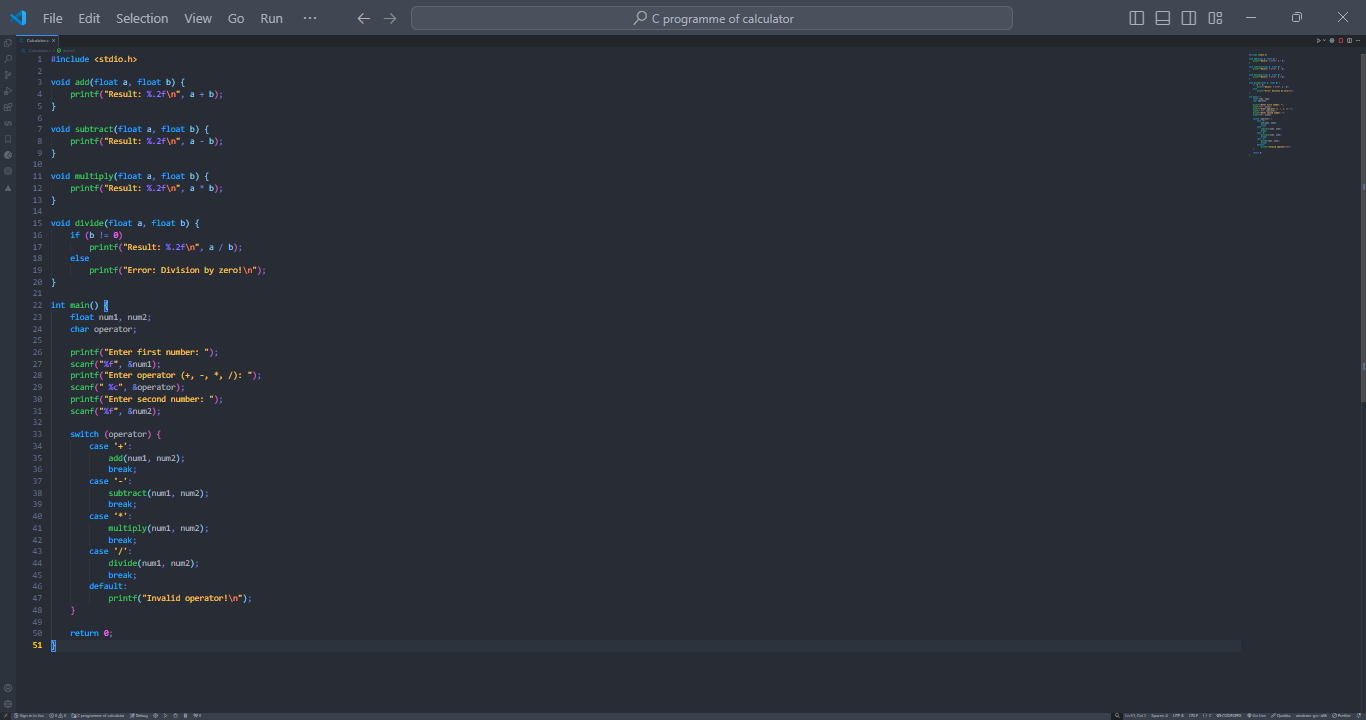
\includegraphics[width=0.5\linewidth]{C-calulator.png}
\end{figure}
\vspace{0.5 cm}

\subsection*{Step 5: Commit the Changes in GitHub Desktop}
1. View changes and enter a commit message.\\
2. Click \texttt{Commit to main}.

\subsection*{Step 6: Publish the Repository}
1. Click \texttt{Publish repository}.\\
2. Choose visibility (public or private).\\
3. Click \texttt{Publish Repository}.

\subsection*{Entry by Sreyash Anand}
\textit{Date: [\today]}\\
% Write your lab notebook entry here.


\section{Steps for GitHub Lab Assignment}

\section*{Brief Steps for Completing the Lab Assignment}

\begin{enumerate}[label=\arabic*.]
    \item \textbf{Clone the Repository:}
    \begin{itemize}
        \item Open GitHub Desktop and use the repository link: \url{https://github.com/GeekAyan/STT}.
        \item Click \textbf{"Clone Repository"} and clone it to your local system.
    \end{itemize}

    \item \textbf{Open the Project in IDE:}
    \begin{itemize}
        \item Open the cloned repository in your preferred IDE (e.g., Visual Studio Code, IntelliJ, PyCharm, etc.).
        \item Follow the instructions from the \texttt{README.md} to install dependencies and run the application.
    \end{itemize}

    \item \textbf{Run the Application:}
    \begin{itemize}
        \item Run the project using the appropriate command (provided in the \texttt{README.md}) to check how the "Submit" button looks and behaves.
    \end{itemize}

    \item \textbf{Rename the Button:}
    \begin{itemize}
        \item Locate the code that defines the "Submit" button (likely in a front-end file, such as HTML, JavaScript, or a GUI framework like Tkinter or JavaFX).
        \item Rename the button text to \textbf{"Chin Tapak Dum Dum"}.
    \end{itemize}

    \item \textbf{Analyze and Fix Button Appearance:}
    \begin{itemize}
        \item After renaming the button, it may appear disproportionate. Adjust the styling in the code:
        \begin{itemize}
            \item Modify the \textbf{CSS} (if a web app) or \textbf{layout properties} (if a desktop app) to increase the button's width, height, font size, or padding.
            \item Test the button until it looks well-proportioned and visually balanced.
        \end{itemize}
    \end{itemize}

    \item \textbf{Run the Application Again:}
    \begin{itemize}
        \item Once the changes are made, run the application again to ensure everything looks good and functions correctly.
    \end{itemize}

    \item \textbf{Create a Pull Request:}
    \begin{itemize}
        \item Push your changes to a new branch in your GitHub account.
        \item Go to the original repository's page on GitHub and create a \textbf{Pull Request} from your branch to the original repository. Add a description of the changes you made.
        \item Submit the pull request for review.
    \end{itemize}

\end{enumerate}

\subsection*{Entry by Ritesh Kumar Shah}
\textit{Date: [\today]}\\
% Write your lab notebook entry here.


\title{Steps to Create CV in LaTeX and Package as Zip}

\section*{Introduction}
This guide will walk you through the steps to create a CV in LaTeX and package all the source files into a zip file for submission.

\section{Step 1: Install LaTeX Environment}
If you haven't already, you need to install a LaTeX editor. Here are some options:
\begin{itemize}
    \item \textbf{Overleaf}: An online LaTeX editor, no installation required.
    \item \textbf{TeXworks}: For Windows.
    \item \textbf{TeXShop}: For macOS.
    \item \textbf{Kile}: For Linux.
\end{itemize}

\section{Step 2: Write Your LaTeX Document}
\begin{enumerate}
    \item \textbf{Open your LaTeX editor}: You can use Overleaf or an installed editor.
    \item \textbf{Create a new project or file}:
    \begin{itemize}
        \item In Overleaf, click \textit{New Project} and choose \textit{Blank Project}.
        \item In local editors, create a \texttt{.tex} file using your LaTeX editor.
    \end{itemize}
    \item \textbf{Write your CV}: Write the LaTeX code for your CV, structuring it with sections like Personal Information, Education, Work Experience, etc.
\end{enumerate}

\section{Step 3: Compile the LaTeX Document}
\begin{enumerate}
    \item \textbf{Compile the \texttt{.tex} file}: 
    \begin{itemize}
        \item In Overleaf, click \textit{Recompile}.
        \item In other editors, look for the \textit{Build} or \textit{Compile} button.
    \end{itemize}
    \item \textbf{Check the output} to ensure everything looks correct.
\end{enumerate}

\section{Step 4: Gather the Necessary Files}
Once the LaTeX file compiles successfully, collect these files:
\begin{itemize}
    \item The \texttt{.tex} file (LaTeX source code).
    \item The compiled PDF.
    \item Any additional files (e.g., \texttt{.cls} files, images, etc.).
\end{itemize}

\section{Step 5: Name the Folder}
Create a folder using the following format:
\begin{verbatim}
Rollno_DeptName_Firstname_CV
\end{verbatim}
For example, if your roll number is \texttt{12345}, department is \texttt{CSE}, and your first name is \texttt{John}, your folder should be named:
\begin{verbatim}
12345_CSE_John_CV
\end{verbatim}

\section{Step 6: Add Files to the Folder}
Move all the required files (the \texttt{.tex} file, the PDF, and any additional files) into the folder you just created.

\section{Step 7: Zip the Folder}
\begin{itemize}
    \item \textbf{Windows}: Right-click the folder and choose \textit{Send to > Compressed (zipped) folder}.
    \item \textbf{macOS}: Right-click the folder and choose \textit{Compress}.
    \item \textbf{Linux}: Right-click the folder, select \textit{Compress}, and choose the \texttt{.zip} format.
\end{itemize}

\section{Step 8: Verify the Zip File}
Before submitting, ensure that:
\begin{itemize}
    \item The zip file name follows the format: \texttt{Rollno\_DeptName\_Firstname\_CV.zip}.
    \item All necessary files (source code, PDF, and other dependencies) are included.
\end{itemize}

\section{Step 9: Upload the Zip File}
Upload the zip file to the required platform (university portal, email, etc.) for submission.


\subsection*{Entry by Sayantani Hansda}
\textit{Date: [\today]}\\
% Write your lab notebook entry here.


\section*{Git Branching and Merging Steps}

\begin{enumerate}
    \item Create a new repository on GitHub named \texttt{git-advanced}.
    \item Clone the repository to your local machine using: 
        \begin{verbatim}
        git clone <repo_url>
        \end{verbatim}
    \item Create a new branch \texttt{feature-1} and switch to it using:
        \begin{verbatim}
        git checkout -b feature-1
        \end{verbatim}
    \item Create a new file \texttt{shared.txt} with the following content:
        \begin{verbatim}
        This is a shared file.
        Line 1: Original text.
        Line 2: Original text.
        \end{verbatim}
    \item Stage and commit the changes with:
        \begin{verbatim}
        git add shared.txt
        git commit -m "Add shared.txt with original text"
        \end{verbatim}
    \item Push the branch to GitHub:
        \begin{verbatim}
        git push -u origin feature-1
        \end{verbatim}
    \item Create a new branch \texttt{feature-2} and switch to it:
        \begin{verbatim}
        git checkout -b feature-2
        \end{verbatim}
    \item Checkout \texttt{shared.txt} from the \texttt{main} branch:
        \begin{verbatim}
        git checkout main -- shared.txt
        \end{verbatim}
    \item Modify the second line in \texttt{shared.txt}:
        \begin{verbatim}
        Line 2: Modified text in feature-2.
        \end{verbatim}
    \item Stage and commit the changes with:
        \begin{verbatim}
        git add shared.txt
        git commit -m "Modify second line in feature-2"
        \end{verbatim}
    \item Push \texttt{feature-2} to GitHub:
        \begin{verbatim}
        git push -u origin feature-2
        \end{verbatim}
    \item Switch back to the \texttt{feature-1} branch:
        \begin{verbatim}
        git checkout feature-1
        \end{verbatim}
    \item Modify the second line in \texttt{shared.txt}:
        \begin{verbatim}
        Line 2: Modified text in feature-1.
        \end{verbatim}
    \item Stage and commit the changes with:
        \begin{verbatim}
        git add shared.txt
        git commit -m "Modify second line in feature-1"
        \end{verbatim}
    \item Push \texttt{feature-1} to GitHub.
    \item Merge \texttt{feature-1} into the \texttt{main} branch:
        \begin{verbatim}
        git checkout main
        git merge feature-1
        \end{verbatim}
    \item Merge \texttt{feature-2} into the \texttt{main} branch (this will cause a conflict):
    \vspace{1 cm}
\begin{figure}[h!]
   \centering
    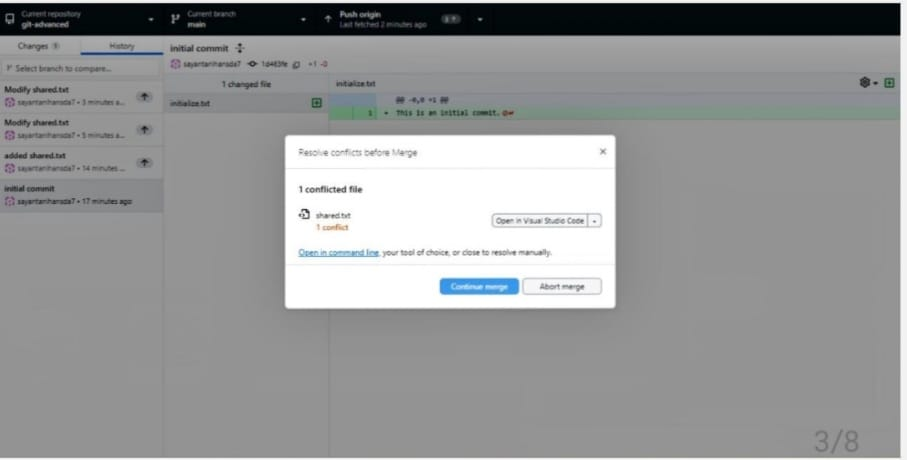
\includegraphics[width=0.5\linewidth]{conflict.jpg}
\end{figure}
\vspace{0.5 cm}
 \vspace{1 cm}
\begin{figure}[h!]
   \centering
    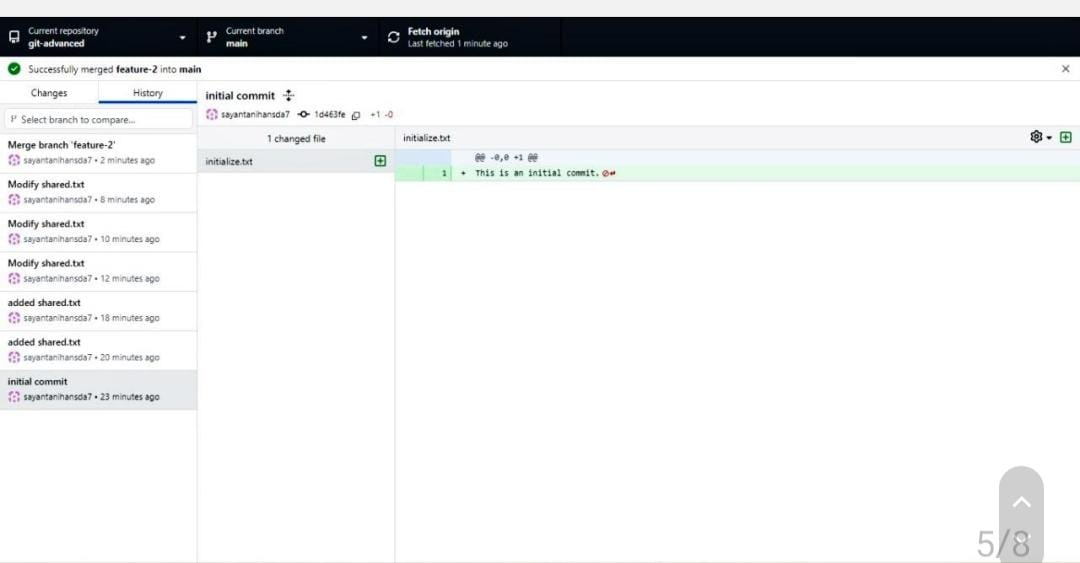
\includegraphics[width=0.5\linewidth]{History.jpg}
\end{figure}
\vspace{0.5 cm}

        \begin{verbatim}
        git merge feature-2
        \end{verbatim}
    \item Resolve the conflict in \texttt{shared.txt}, then stage and commit the resolution:
        \begin{verbatim}
        git add shared.txt
        git commit -m "Resolve conflict between feature-1 and feature-2"
        \end{verbatim}
    \item Push the resolved \texttt{main} branch:
        \begin{verbatim}
        git push
        \end{verbatim}
    \item Delete both feature branches:
     \vspace{1 cm}
\begin{figure}[h!]
   \centering
    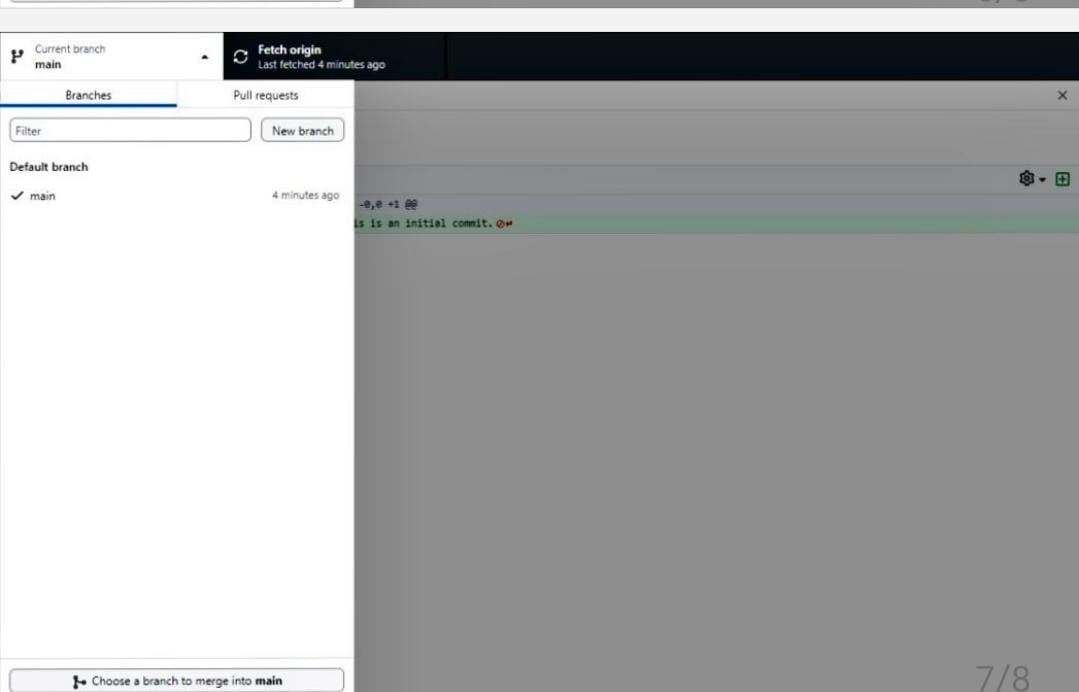
\includegraphics[width=0.5\linewidth]{Delete.jpg}
\end{figure}
\vspace{0.5 cm}
        \begin{verbatim}
        
        git branch -d feature-1
        git branch -d feature-2
        git push origin --delete feature-1
        git push origin --delete feature-2
        \end{verbatim}
\end{enumerate}

\end{document}
